\subsection*{Borúwky} % (fold)
\label{sub:borúwky}

\begin{multicols}{1}

STAVEBKA:-)!\\
Jednoho dne jsme nastopili do onoho vlaku a odjeli na měsíc na jedno velmi neůtulné místečko k Ostrovci. Toto (pole) Louka byla velmi porostlá porostem. ze začátku se nám opoždila dovážka vody a mi jsme trpěli žízní. To byly asi 3 hodiny. Mezitím jsme dělali kolíky a matroš na kuchyň. Postavil se sněmák, nanosily bedny. Ustlali jsme si a dokonce jsme vyrazli i k “rybníku„ se umýt. Jstli vy co si to čtete si myslíte že jsme šli za sucha, světla, a tepla tak se šíleně pletete. Šli jsme za deště, zimy a za šera. Když jsme dorazili k okomu místu byla voda docela teplá. Když jsme se vraceli tak nám ostatní trocju utekli a já a Kája jsme za nimi v té tmě běželi po silnici. Druhého dne jsme pokračovali ve stavbě. Voda konečně dorazila a mi jsme se pustili do dalších prací. Mi jsme s Kájou a s Bendou kopali sklípek. Docela jsme si mákli a další den nás boleli záda. Stavba pokročila a mi už jsme měli postavenou kuchyň, latry a sklípek. Dále jsme vykopávali táboroví kruh O. Nejaký vedoucí (Alvis) nám ho zkrytizoval a na úkor toho jsme to museli velkou vrstvou zakopat. Všechno už bylo hotovo v ten onen den kdy ostatní přijeli. (Tedy maruška a Eskymáci s Urzony). To byla úleva (Jo a šlapali jsme bahno :) Hmm) ale to zas Jindy :)

\podpis{Jumbo:)}
	

MANÉVRY\\
Jednoho dne se na nástence objevil nápis MANÉVRY všichni si z toho dělali srandu ale odpoledne nás zavolala Cucumbrie a museli jsme odejít. Naše čtyř člená družinka (Jeden člen zůstal v táboře) šla do Ostrovce kde jsme potkali Debat a Šerifa. Spali jsme někde u Dědovic a ráno jsme museli jít asi pět kiláků.


Po cestě jsme neůzpěšně brodili takže jsme měli mokré boty ale dohonili jsme vedoucí a do cíle jsme došli asi o dvě hodiny dřív. Spali jsme kousek od nějakého hradu i s ostatníma družinkama protože jsme ráno měli dojít k hradu. 


Ráno jsme šli na hrad a na prohlídku a potom jsme šli k vodě kde přijeli piráti. Potom jsme dostali kousek mapi od Bezvousky a mohli jsme jít do tábora.

\podpis{Maruška}

VORVO\\
Byl nástup. Řekli nám že se máme převlíknout do oblečení které se může ušpinit. Potom nám svázali ruce ke klacku. Když jsme byli svázány odvlekli nás do vyschlého potoku. Všude byli spadlé stromy bahno a klacky. Museli jsme prolézt kus toho vyschlého potoku. Skoro všichni měli po kotníky bahno a ještě k tomu jsme měli pořád svázané ruce! 


Když jsme vylezli zavázali nám oči a odvlekli na další louku kde po nás házeli mouku. Potom jsme šli k pumpě u které nás nabarvili na modro. Když jsme byli nabarvený tak nám nabarvili zeleně vlasy. Potom jsme utekli k TP A vedle nich jsme hráli hru při které jsme se honili. Potom jsme šli spátky za ostatními. Byl to hustý pocit jak se na nás všichni koukali. A naše vlasy vypadali báječně!

\podpis{Kája}

\end{multicols}

\begin{center}

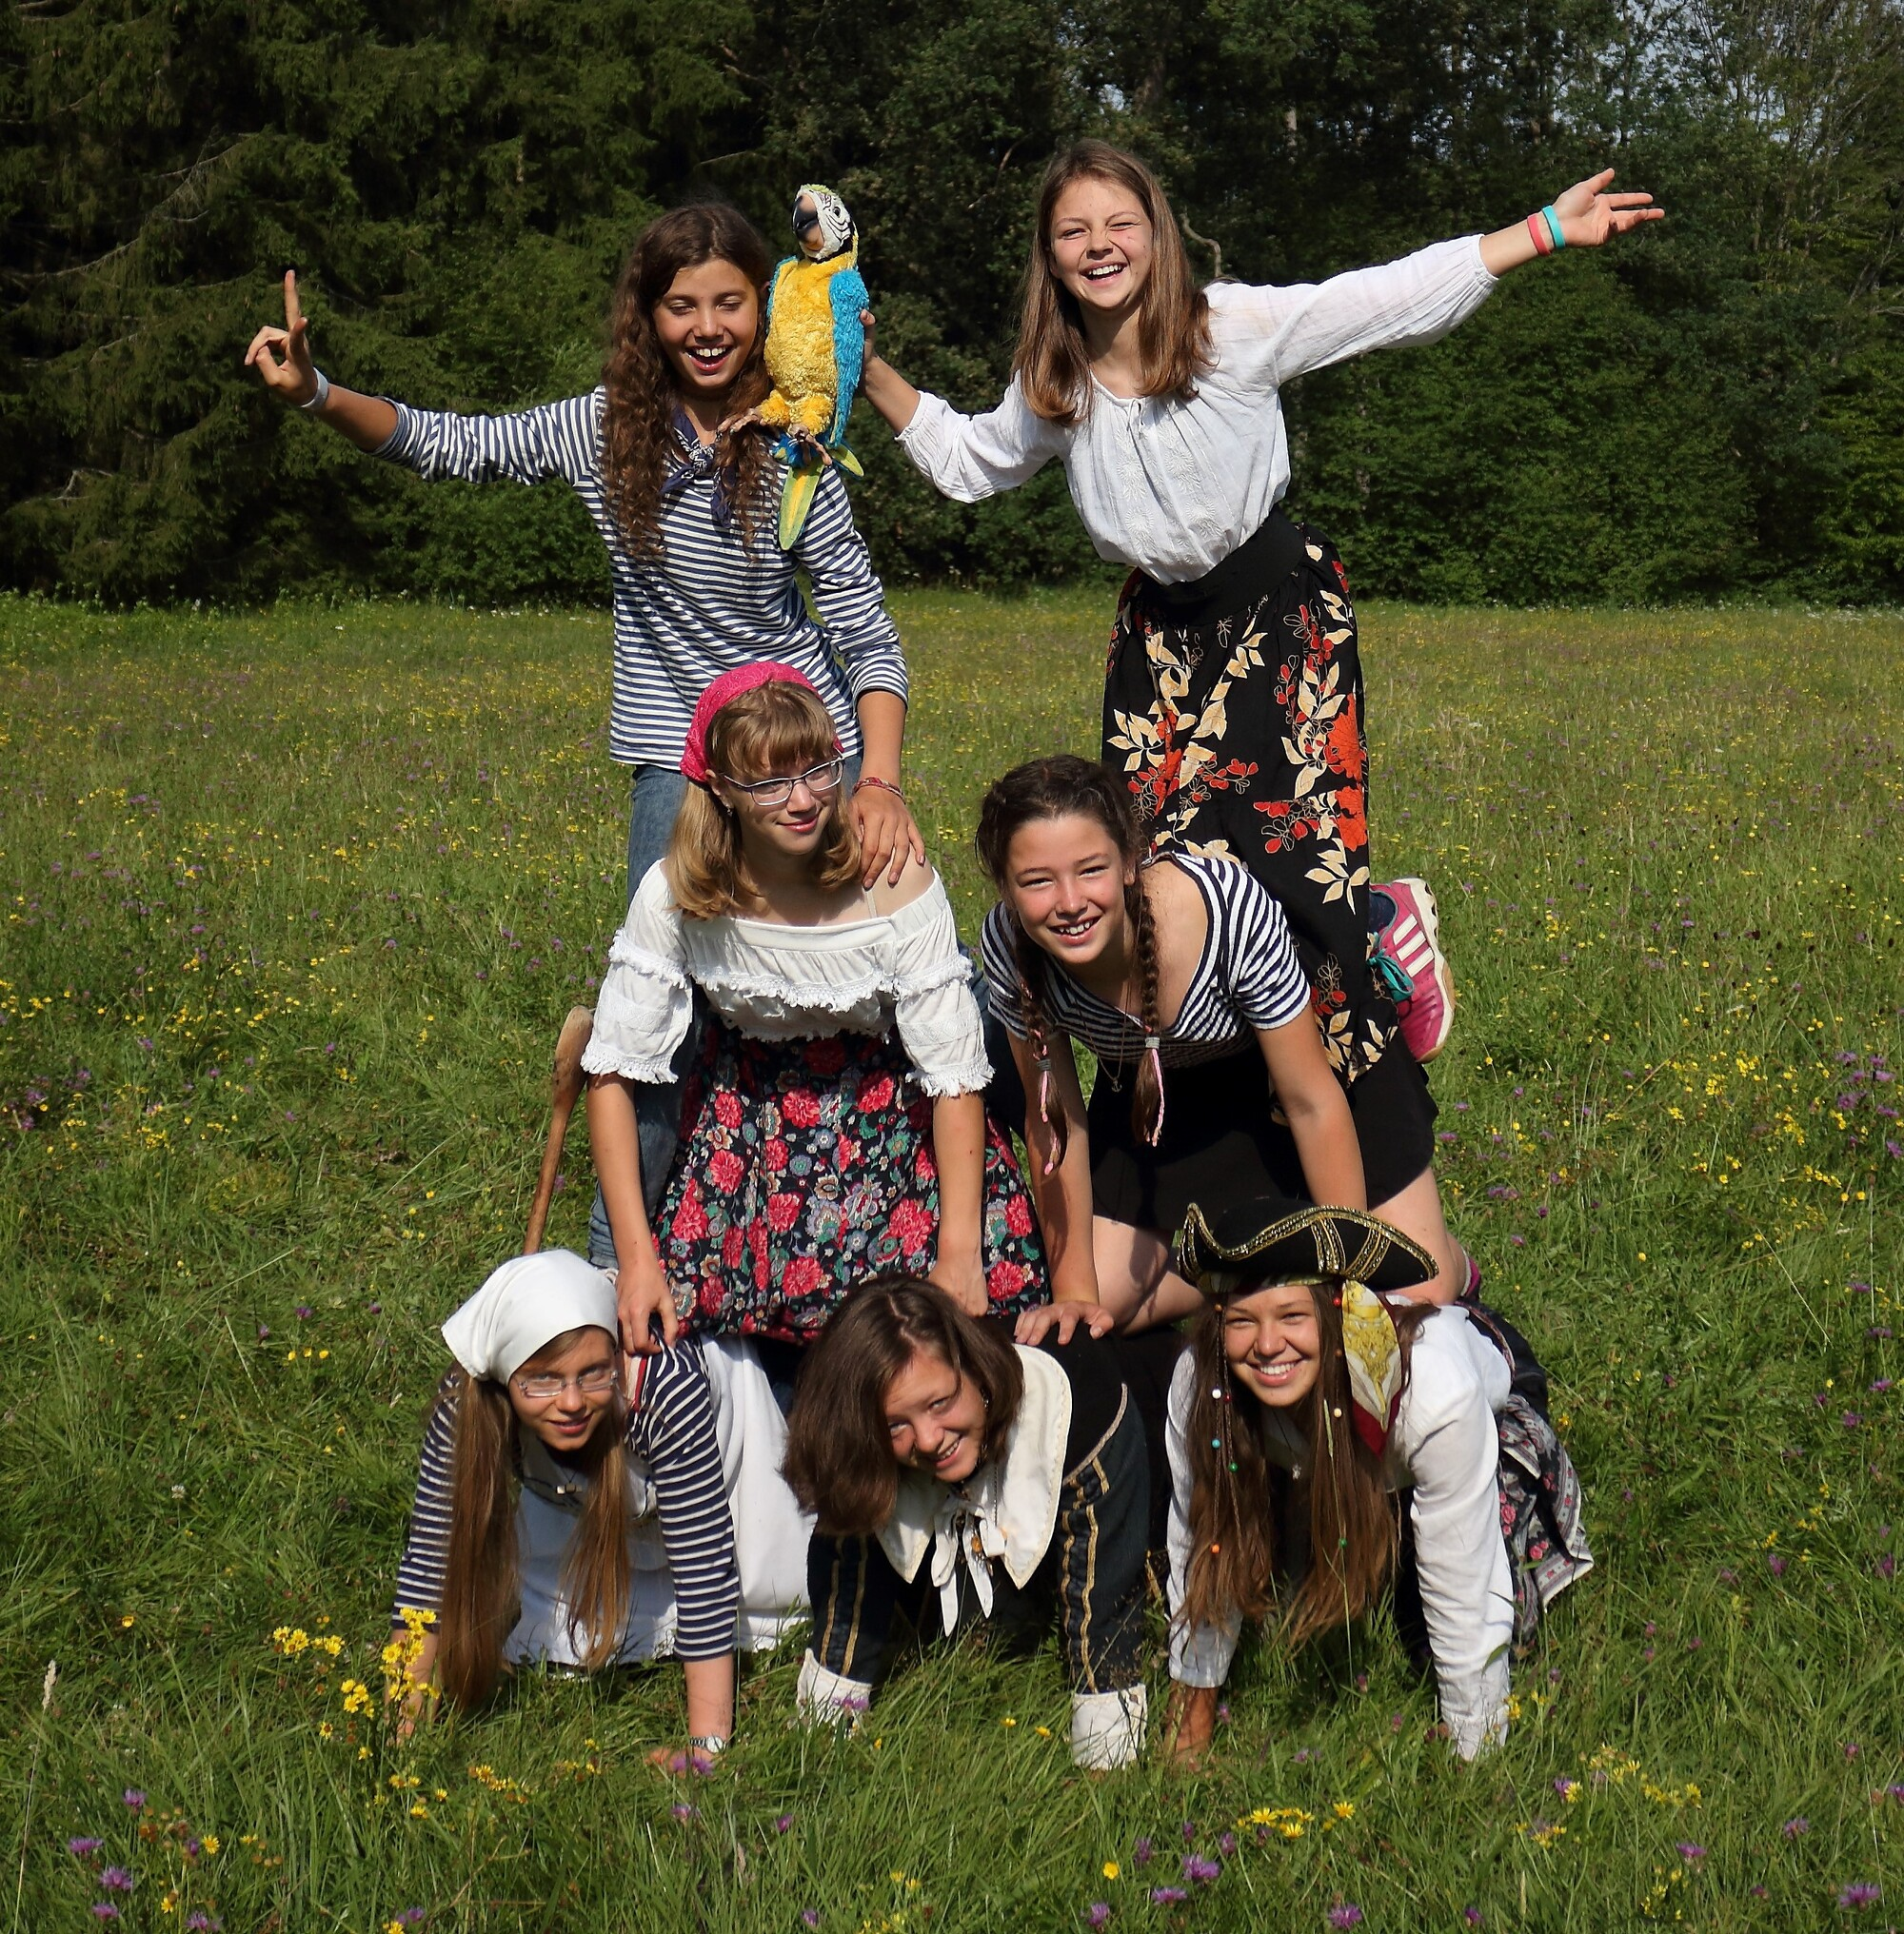
\includegraphics[width=9cm]{img/druziny/boruwky.jpg}

\end{center}

\clearpage


% subsection borúwky (end)
